\chapter{Revue de la littérature}
\begin{onehalfspace}

\hspace{0.65cm}La détection multi-visages sur plateforme mobile pour le marquage de présence académique représente un défi technique complexe, situé à l'intersection de plusieurs domaines de recherche. Cette revue examine l'évolution des approches et justifie les choix technologiques conduisant à notre solution.


\section{Vision par Ordinateur et reconnaissance de Formes}

\hspace{0.65cm}La vision par ordinateur et la reconnaissance de formes se divisent en trois approches majeures pour l'analyse d'images numériques : l'analyse de scènes, la compréhension d'images et les systèmes biométriques. Chacune de ces approches propose une perspective différente pour le traitement de l'information visuelle.

\hspace{0.65cm}L'analyse de scènes (Scene Analysis) se concentre sur la compréhension globale de l'environnement visuel. Cette approche segmente l'image en régions sémantiques et interprète les relations spatiales entre les objets \cite{Mohammed2024InsightsII}. Dans un contexte de classe, elle permettrait de comprendre l'agencement général de la salle et la disposition des étudiants. Cependant, cette approche globale, bien que riche en informations contextuelles, s'avère trop générale et computationnellement coûteuse pour notre objectif spécifique de détection de visages. Les modèles d'analyse de scènes nécessitent généralement plusieurs gigaoctets de mémoire et des temps de traitement dépassant la seconde, les rendant inadaptés aux contraintes mobiles.

\hspace{0.65cm}La compréhension d'images (Image Understanding) vise à extraire une interprétation sémantique complète du contenu visuel. Cette approche identifie non seulement les objets présents mais aussi leurs attributs et leurs interactions \cite{Astolfi2021Syntactic}. Appliquée à notre contexte, elle fournirait des informations sur l'attention des étudiants, leur posture, ou même leur niveau d'engagement. Bien que ces informations soient potentiellement utiles, cette approche généraliste nécessite des modèles complexes (>500MB) et un temps de traitement significatif (>2s par image), dépassant largement nos contraintes de ressources mobiles.

\hspace{0.65cm}Les systèmes biométriques représentent l'approche la plus spécialisée, se concentrant spécifiquement sur l'identification des caractéristiques uniques des individus. Cette spécialisation permet une optimisation poussée des algorithmes pour la détection et la reconnaissance des traits biométriques. Dans notre contexte de marquage de présence, cette approche offre plusieurs avantages décisifs : un pipeline de traitement optimisé pour les visages (mémoire <100MB), une rapidité d'exécution adaptée au mobile (latence <500ms pour 30 visages), et une précision élevée en conditions réelles (>95\% de détections correctes).

\hspace{0.65cm}Le choix des systèmes biométriques comme approche principale se justifie donc par trois facteurs clés : leur spécialisation qui permet une optimisation poussée pour les dispositifs mobiles, leur efficacité dans le traitement simultané de multiples sujets, et leur robustesse aux conditions variables d'une salle de classe. Cette approche ouvre également la voie à une intégration naturelle des fonctionnalités de reconnaissance pour l'identification des étudiants, aspect crucial de notre système de marquage de présence.



\section{Systèmes Biométriques}
\hspace{0.65cm} Dans le domaine des systèmes biométriques, trois modalités principales se distinguent pour l'identification des individus : l'analyse faciale (Face Analysis), la reconnaissance d'empreintes digitales (Fingerprint Recognition) et la reconnaissance de l'iris (Iris Recognition). Ces approches diffèrent fondamentalement dans leur mise en œuvre et leur adéquation avec un contexte de marquage de présence académique.

\hspace{0.65cm} La reconnaissance d'empreintes digitales représente la modalité biométrique la plus mature technologiquement. Cette approche, basée sur l'extraction des minuties uniques présentes dans les dermatoglyphes, atteint des taux de reconnaissance exceptionnels (FAR < 0.001\%, FRR < 1\%). Cependant, son déploiement dans un contexte académique se heurte à des limitations pratiques majeures : le traitement séquentiel imposé par la nécessité d'un contact physique avec le capteur entraîne des temps d'acquisition prohibitifs pour un groupe d'étudiants (2-3 secondes par personne), rendant impossible un marquage de présence rapide pour une classe entière.

\hspace{0.65cm} La reconnaissance de l'iris offre une précision encore supérieure grâce à la richesse des motifs de l'iris humain (FAR < 0.0001\%, FRR < 0.5\%). Cette approche sans contact pourrait sembler plus adaptée à un environnement académique. Néanmoins, elle requiert des conditions d'acquisition très spécifiques : une distance de capture précise (20-35cm), un éclairage contrôlé et une coopération active du sujet pour l'alignement de l'œil. Ces contraintes rendent son utilisation impraticable pour la capture simultanée de multiples étudiants dans une salle de classe.

\hspace{0.65cm}L'analyse faciale émerge comme la solution idéale pour notre contexte spécifique. Cette approche permet une capture à distance naturelle (1-8m), sans contact et surtout simultanée pour multiple sujets. Les systèmes modernes d'analyse faciale atteignent des performances remarquables (précision > 95\%) tout en maintenant une flexibilité opérationnelle essentielle en environnement académique. La capacité de traitement parallèle permet l'analyse d'une classe entière en une seule capture (< 500ms pour 30+ visages), offrant une efficacité incomparable pour le marquage de présence.


\section{Analyse Faciale}
\hspace{0.65cm}L'analyse faciale comprend trois domaines complémentaires : la détection de visages, la reconnaissance faciale et l'analyse d'expressions. La reconnaissance faciale elle-même se divise en deux tâches distinctes : la vérification, qui compare une paire de visages pour déterminer s'ils appartiennent à la même personne, et l'identification, qui recherche l'identité d'un visage dans une base de données d'individus connus.

\hspace{0.65cm} Notre système de marquage de présence académique vise ultimement l'identification à grande échelle, où chaque visage détecté devra être comparé à une base de données d'étudiants. Cette tâche est particulièrement exigeante car sa complexité augmente avec la taille de la base de données et le nombre de visages à traiter simultanément. Cependant, avant même d'aborder ces défis d'identification, une détection robuste et précise des visages dans l'image est primordiale \cite{186Текстстатті46511020230930}.

\hspace{0.65cm}L'analyse d'expressions faciales pousse l'interprétation plus loin en décodant les émotions et les micro-expressions des sujets. Bien que potentiellement intéressante pour l'analyse de l'engagement des étudiants, cette approche ajoute une complexité computationnelle injustifiée (>300ms par visage) pour notre objectif premier de marquage de présence. Elle nécessite également une résolution d'image plus élevée, augmentant les besoins en ressources.

\hspace{0.65cm} La détection multi-visages sur une image statique constitue donc notre priorité initiale. Dans un environnement de classe, où plusieurs dizaines d'étudiants peuvent être présents simultanément, la capacité à détecter précisément tous les visages, malgré les variations de distance (1-8 mètres), d'éclairage et de pose, est cruciale. Les détecteurs modernes, optimisés pour ces scénarios complexes, maintiennent des performances élevées (>90\% sur WIDER FACE) tout en respectant les contraintes mobiles (50MB de mémoire, 30ms par frame).

\hspace{0.65cm} Cette focalisation sur la détection multi-visages est importante car, même l'algorithme d'identification le plus sophistiqué ne peut compenser une détection manquée ou imprécise. À grande échelle, chaque erreur de détection se traduit potentiellement par une absence non comptabilisée. De plus, la qualité de la détection influence directement la précision de l'identification future : des visages bien détectés, correctement alignés et normalisés augmentent significativement les chances d'une identification réussie.

\hspace{0.65cm} Notre approche établit ainsi une base solide pour l'évolution du système. En garantissant d'abord une détection multi-visages fiable sur images statiques, nous préparons le terrain pour une implémentation future de l'identification à grande échelle. Cette stratégie progressive permet de maintenir la qualité du service de base (le marquage de présence) tout en ouvrant la voie à des fonctionnalités plus avancées d'identification.

\section{Détection et Suivi de Visages}
\hspace{0.65cm} La détection et le suivi de visages constituent un pilier fondamental de l'analyse faciale. Ce domaine vise à localiser et suivre avec précision les visages dans une image ou une séquence vidéo, posant des défis spécifiques qui ont conduit à l'évolution des approches de résolution.

\hspace{ 0.65cm} Les défis fondamentaux de la détection de visages se manifestent à plusieurs niveaux. Les variations intrinsèques incluent les changements d'expressions faciales, les différentes poses et les attributs variables comme la présence de lunettes ou de masques. Les conditions externes ajoutent des complexités supplémentaires avec les variations d'éclairage, les occlusions partielles et les différentes échelles de visages dans l'image. Dans un contexte mobile, ces défis se conjuguent avec des contraintes système strictes : nécessité d'un traitement temps réel, ressources limitées et exigence de haute précision.

\hspace{0.65cm} La réponse à ces défis a évolué à travers deux générations d'approches. L'approche classique repose sur l'analyse directe des pixels et l'utilisation de règles prédéfinies, comme la recherche de motifs d'intensité caractéristiques des visages. Des techniques comme le processus de Viola-Jones, combiné avec l'analyse en composantes principales (PCA), sont utilisées pour améliorer la précision de la détection des visages \cite{Mamieva2023Improved}.

\hspace{0.65cm} L'introduction de l'apprentissage automatique a permis une meilleure adaptation aux variations naturelles en apprenant à partir d'exemples. L'apprentissage profond, dernière évolution majeure, apporte une capacité sans précédent à gérer la complexité des scènes réelles.

\section{Apprentissage Automatique}
\hspace{0.65cm} L'apprentissage automatique marque une rupture fondamentale dans la détection de visages en introduisant la capacité d'apprendre à partir des données plutôt que de suivre des règles explicites. Cette approche se caractérise par deux composantes essentielles : l'extraction de caractéristiques et la classification.

\hspace{0.65cm} L'extraction de caractéristiques vise à représenter l'image de manière compacte et discriminante. Ce processus consiste à extraire des informations significatives d'une image, telles que les bords, les textures et les formes, qui peuvent être utilisées pour identifier un visage. Des descripteurs comme HOG (Histograms of Oriented Gradients) capturent la distribution des gradients d'intensité, tandis que LBP (Local Binary Patterns) encode les motifs de texture locaux. Ces caractéristiques, bien que conçues manuellement (handcrafted), offrent une certaine robustesse aux variations d'éclairage et de pose.

\hspace{0.65cm} La classification utilise ces caractéristiques pour décider de la présence ou non d'un visage. Les classifieurs comme SVM (Support Vector Machines) ou AdaBoost apprennent à partir d'exemples à distinguer les visages des non-visages. Cette approche permet d'atteindre des performances de l'ordre de 75-80\% dans des conditions variables, mais reste limitée par la nature prédéfinie des caractéristiques utilisées.


\section{Architectures d'apprentissage profond}
\hspace{0.65cm} L'apprentissage profond révolutionne la détection de visages en unifiant l'extraction de caractéristiques et la classification dans un système de bout en bout. Les réseaux de neurones convolutifs (CNN) sont au coeur de cette révolution, avec trois principales familles d'architectures : single-stage, multi-stage et basées sur l'attention

\hspace{0.65cm} Les architectures single-stage, telles que YOLO et SSD, sont conçues pour un équilibre optimal entre précision et vitesse. Elles effectuent la détection en une seule étape, ce qui les rend adaptées aux applications en temps réel. Par exemple, YOLO-FaceV2 améliore la détection en temps réel en utilisant des modules d'attention pour gérer les visages petits et partiellement occultés \cite{yu2022yolofacev2scaleocclusionaware}. L'efficacité computationnelle de cette architecture, combinée à sa capacité à maintenir une précision élevée (>95\%), en fait une solution particulièrement adaptée aux contraintes mobiles.

\hspace{0.65cm}Les architectures multi-stage, comme Faster R-CNN, impliquent plusieurs étapes de traitement, ce qui peut améliorer la précision au détriment de la vitesse. Ces modèles sont souvent utilisés dans des contextes où la précision est plus critique que la rapidité \cite{186Текстстатті46511020230930}. Bien que cette approche atteigne une précision remarquable (>98\%), la latence cumulée des différents étages et les ressources requises la rendent moins adaptée au déploiement mobile.

\hspace{0.65cm} Les modèles basés sur l'attention, tels que ceux utilisant des mécanismes multi-attention, se concentrent sur les caractéristiques anormales des visages pour améliorer la détection, notamment dans les cas de manipulation de visages. Ces modèles exploitent des mécanismes d'attention pour extraire des caractéristiques détaillées et améliorer la performance de détection \cite{Cao2021Face}. Malgré leur capacité impressionnante à capturer des dépendances à longue distance, leur coût computationnel quadratique les exclut actuellement des applications mobiles temps réel.

\hspace{0.65cm} Le choix d'une architecture single-stage pour notre système se justifie par plusieurs facteurs critiques. Son pipeline unifié minimise la latence globale, crucial pour le traitement temps réel. Sa gestion native des multi-échelles via le FPN répond parfaitement aux variations de distance dans une salle de classe. Enfin, sa simplicité architecturale facilite les optimisations pour plateformes mobiles, permettant un déploiement efficace avec des ressources limitées.

\section{Architecture single-stage}
 Dans un système de detection de visage basé sur l'apprentissage profond, les architectures single-stage apdatent généralement  trois parties principales: le réseau dorsal, le cou et la tête \cite{186Текстстатті46511020230930}
\begin{itemize}
     \item Réseau dorsal (backbone): Il s'agit d'un réseau neuronal convolutif pré-entraîné (par exemple, ResNet, VGG) qui extrait les caractéristiques de l'image d'entrée
     \item Cou (neck): Cette partie combine et affine les caractéristiques extraites par le réseau dorsal, souvent en utilisant des structures pyramidales comme le Feature Pyramid Network (FPN).
     \item Tête (head): La tête est responsable de la prédiction finale, qui comprend la localisation du visage (boîte englobante) et la classification (visage ou non-visage).

\end{itemize}

\section{Etat de l'art}

\hspace{0.65cm} La détection de visages sur plateformes mobiles constitue un défi majeur en vision par ordinateur, particulièrement pour les applications de vérification de présence en salle nécessitant une détection multi-visages fiable en conditions d'éclairage intérieur variables. L'évolution des architectures deep learning single-stage reflète cette recherche de compromis, passant progressivement d'architectures computationnellement lourdes à des solutions optimisées pour le déploiement mobile hors ligne..

\hspace{0.65cm} \cite{Liu2015SSDSS}  établissent les fondements avec SSD (Single Shot MultiBox Detector), conçu initialement comme détecteur d'objets générique avant son adaptation à la détection de visages. L'architecture utilise VGG-16 comme réseau dorsal, choisi pour son efficacité prouvée dans l'extraction de caractéristiques discriminantes. SSD se distingue par l'absence de cou distinct, privilégiant une approche directe d'utilisation des cartes de caractéristiques, et emploie une tête de détection basée sur un système d'ancres multi-échelles. Le modèle atteint 74,3\% mAP (SSD300) et 76,9\% (SSD512) sur VOC2007 à 59 FPS sur Nvidia Titan X. Cependant, sa complexité computationnelle et sa sensibilité aux variations d'illumination limitent son application dans un contexte mobile.

\hspace{0.65cm} Pour répondre à ces limitations, \cite{Li2023SinglestageFD} ont développé ESSFD, introduisant une architecture plus sophistiquée. Leur réseau dorsal ResNet-D optimisé améliore l'extraction de caractéristiques discriminantes grâce à une architecture résiduelle profonde. L'innovation majeure réside dans leur cou intégrant des convolutions atrous, permettant une capture multi-échelles efficace sans augmentation excessive des paramètres. Leur approche atteint des performances remarquables sur WIDER FACE avec 95.373\%, 93.788\% et 84.223\% respectivement sur les niveaux Easy, Medium et Hard. Néanmoins, ESSFD nécessite 152,94 GFLOPs et 77 million de paramètres. Bien qu'ESSFD améliore la précision de la détection des visages, son coût computationnel et sa taille de modèle restent élevés, ce qui peut limiter son utilisation sur les appareils mobiles.

\hspace{0.65cm} \cite{Deng2019RetinaFaceSD} ont développé RetinaFace avec une approche architecturale innovante. Leur réseau dorsal s'appuie sur un ResNet-152 pré-entraîné sur ImageNet-11k, permettant une extraction plus robuste des caractéristiques discriminantes et une meilleure distinction des visages en conditions complexes. Le cou de l'architecture introduit un réseau pyramidal de caractéristiques avec connexions descendantes et latérales, fusionnant efficacement les informations des différentes étapes résiduelles. Cette approche améliore significativement la gestion multi-échelle, précédemment limitée dans ESSFD. Leur tête de détection intègre des modules de contexte indépendants sur cinq niveaux pyramidaux, exploitant la richesse des caractéristiques extraites. Les expérimentations démontrent une précision de RetinaFace obtient 94,653\%, 93,007\% et 82,357\%respectivement sur les niveaux Easy, Medium et Hard de WIDERFACE. RetinaFace utilise 150,79 GFLOPs et 57 million de paramètres. L'architecture révèle des limitations persistantes dans la gestion des visages fortement occultés et des conditions d'illumination variables. De plus une architectures plus légères est necessaire pour son utilisation sur les appareils mobiles.

\hspace{0.65cm} SCRFD-2.5GF a été conçu par \cite{Guo2021SampleAC} comme un détecteur de visage ultraléger et efficace, particulièrement adapté aux appareils embarqués et mobiles avec des ressources limitées. L'architecture utilise ResNet-18 comme réseau dorsal, un choix motivé par sa légèreté et son efficacité computationnelle tout en maintenant une bonne capacité d'extraction de caractéristiques, ce qui est crucial pour les applications où les ressources sont limitées. Au niveau du cou, le modèle emploie un FPN (Feature Pyramid Network) standard, choisi pour sa capacité à combiner efficacement les caractéristiques à différentes résolutions, ce qui est essentiel pour la détection de visages de tailles variables. La tête de détection utilise une stratégie d'ancrage dense, permettant une meilleure couverture des différentes tailles et rapports d'aspect des visages, ce qui améliore particulièrement la détection des petits visages. En termes de performances sur WIDERFACE, SCRFD-2.5GF atteint des résultats impressionnants avec 93,78\%, 92,16\% et 77,87\% de précision sur les sous-ensembles Easy, Medium et Hard respectivement, tout en maintenant une efficacité remarquable avec seulement 2,5 GFLOPs et 3,8 millions de paramètres. Cependant, le modèle présente certaines limitations, notamment des performances plus faibles sur le sous-ensemble Hard comparé à des modèles plus lourds, une possible sensibilité aux variations d'illumination, et une dépendance à la stratégie d'ancrage dense qui pourrait être optimisée pour améliorer davantage l'efficacité du modèle. De plus cette approche pourrait être sensible aux variations de résolution et de ratio d'aspect de l'image. Si le format d'image utilisé pour l'application diffère de celui utilisé lors de l'entraînement. Ainis des ajustements et une optimisation supplémentaires pourraient être nécessaires pour maintenir des performances optimales.


\hspace{0.65cm} YOLOv5n a été conçu par \cite{Qi2021YOLO5FaceWR} comme un détecteur de visage léger et efficace, spécifiquement optimisé pour les applications sur appareils embarqués et mobiles avec des ressources limitées. L'architecture utilise ShuffleNetV2 comme réseau dorsal, un choix justifié par son efficacité computationnelle grâce à l'utilisation de convolutions en profondeur et du shuffling de canaux, permettant de réduire la complexité tout en maintenant de bonnes performances. Au niveau du cou, le modèle combine SPP (Spatial Pyramid Pooling) et PAN (Path Aggregation Network), où SPP permet l'extraction de caractéristiques multi-échelles essentielles pour la détection de visages de différentes tailles, tandis que PAN assure une fusion efficace des caractéristiques à différents niveaux pour améliorer la précision de localisation et de classification. La tête de détection intègre non seulement la régression des boîtes englobantes et la classification des visages, mais aussi une tête supplémentaire pour la régression des points de repère du visage utilisant la fonction de perte Wing, reconnue pour sa robustesse aux valeurs aberrantes. Sur WIDERFACE, YOLOv5n atteint des performances impressionnantes avec 93,61\%, 91,54\% et 80,53\% de précision sur les sous-ensembles Easy, Medium et Hard respectivement, tout en maintenant une efficacité remarquable avec seulement 1,726 million de paramètres et 2,111 GFLOPs. Cependant, le modèle présente des limitations, notamment dans la détection des très petits visages, la robustesse aux conditions d'éclairage difficiles et la gestion des visages partiellement occultés, suggérant des pistes d'amélioration potentielles comme l'ajout de couches à plus haute résolution, l'utilisation de techniques d'illumination invariante et l'implémentation de mécanismes d'attention plus avancés.


\hspace{0.65cm} FDLite a été conçu par \cite{Aggarwal2024FDLiteAS}  comme un détecteur de visage ultra-léger optimisé pour les applications en temps réel sur les appareils de bord, avec l'objectif de minimiser les coûts de calcul sans compromettre la précision. L'architecture utilise BLite comme réseau dorsal, un choix justifié par son extrême légèreté (0,167 million de paramètres, 0,52 GFLOPs) tout en maintenant des performances compétitives par rapport aux réseaux plus volumineux. Au niveau du cou, FDLite emploie un FPN (Feature Pyramid Network) pour sa capacité à combiner efficacement les caractéristiques à différentes échelles et à améliorer les caractéristiques des couches inférieures avec les informations sémantiques des couches supérieures, ce qui est particulièrement bénéfique pour la détection des petits visages. La tête de détection se distingue par l'utilisation de deux pertes multi-tâches indépendantes, chacune comprenant trois sous-réseaux dédiés à la classification des visages, la localisation des boîtes englobantes et la détection des points d'intérêt du visage, permettant ainsi un apprentissage plus précis et robuste. Sur WIDER FACE, FDLite atteint des performances impressionnantes avec 92,3\%, 89,\% et 82,2\% de précision sur les sous-ensembles Easy, Medium et Hard respectivement, tout en maintenant une efficacité remarquable avec seulement 0,26 million de paramètres et 0,94 GFLOPs. Cependant, le modèle présente certaines limitations, notamment une sensibilité aux variations de pose et d'illumination, une possible optimisation de l'architecture du cou en explorant des alternatives au FPN, et le potentiel d'amélioration via l'utilisation de fonctions de perte plus avancées comme la Focal Loss ou la GIoU Loss.

\hspace{0.65cm} \cite{electronics13214184} ont introduit ADYOLOv5-Face, spécifiquement pour améliorer la détection des petits visages, une limitation majeure des modèles YOLO légers. L'architecture utilise CSPDarknet53 comme réseau dorsal, un choix justifié par son excellent compromis entre précision et coût computationnel, faisant de lui une base solide pour la détection de visages. Au niveau du cou, ADYOLOv5-Face innove en remplaçant le FPN traditionnel par un mécanisme Gather-and-Distribute (GD), permettant une transmission plus efficace des informations entre les couches et une meilleure fusion des caractéristiques sémantiques profondes avec les caractéristiques de bas niveau, ce qui améliore significativement la détection des petits visages. La tête de détection comprend quatre têtes de prédiction, dont une spécifiquement optimisée pour les petits visages (Head1) générée à partir de la carte de caractéristiques B2, ce qui améliore considérablement les performances sur les petits visages malgré un léger surcoût computationnel. Sur WIDERFACE, le modèle obtient des résultats impressionnants avec 94,80\%, 93,77\% et 84,37\% de précision sur les sous-ensembles Easy, Medium et Hard respectivement, tout en maintenant une efficacité raisonnable avec 10,123 millions de paramètres et 22,8 GFLOPs. Cependant, le modèle présente encore des limites, notamment sa complexité computationnelle plus élevée que le YOLOv5 de base, des performances potentiellement limitées sur des ensembles de données plus complexes, et la possibilité d'optimiser davantage l'architecture du cou pour la détection des petits visages.

\begin{xltabular}{\textwidth}{>{\RaggedRight\arraybackslash}p{3cm} >{\centering\arraybackslash}p{2cm} >{\centering\arraybackslash}p{2cm} >{\centering\arraybackslash}p{2cm} >{\centering\arraybackslash}p{2cm} >{\centering\arraybackslash}p{2cm} >{\centering\arraybackslash}p{2cm}}
\caption{Analyse comparative des approches de détection de visages triées par mAP, Paramètres et GFLOPs (ordre décroissant)}
\label{tab:comparative-face-detection-sorted-multiple} \\

\toprule
\textbf{Détecteur de visages} & \textbf{Easy (\%)} & \textbf{Medium (\%)} & \textbf{Hard (\%)} & \textbf{mAP (\%)} & \textbf{Paramètres (M)} & \textbf{GFLOPs} \\
\midrule
\endfirsthead

\multicolumn{7}{c}{\tablename\ \thetable{} -- Suite} \\
\toprule
\textbf{Détecteur de visages} & \textbf{Easy (\%)} & \textbf{Medium (\%)} & \textbf{Hard (\%)} & \textbf{mAP (\%)} & \textbf{Paramètres (M)} & \textbf{GFLOPs} \\
\midrule
\endhead

\midrule[\heavyrulewidth]
\multicolumn{7}{r}{\footnotesize Suite page suivante} \\
\endfoot

\bottomrule
\endlastfoot

RetinaFace (ResNet-152) & 94.65 & 93.01 & 82.36 & 90.01 & 57.0 & 150.79 \\
\midrule

ADYOLOv5-Face (CSPDarknet53) & 94.80 & 93.77 & 84.37 & 91.65 & 10.123 & 22.8 \\
\midrule

YOLOv5s (CSPDarknet53) & 94.30 & 93.10 & 80.20 & 89.87 & 7.1 & 16.4 \\
\midrule

SCRFD-2.5GF (ResNet-18) & 93.78 & 92.16 & 77.87 & 87.93 & 0.67 & 2.53 \\
\midrule

YOLOv5n (ShuffleNetV2) & 93.61 & 91.54 & 80.53 & 88.56 & 1.726 & 2.111 \\
\midrule

FDLite (BLite) & 92.30 & 89.90 & 82.20 & 88.13 & 0.26 & 0.94 \\

\end{xltabular}


\begin{figure}[H]
\centering
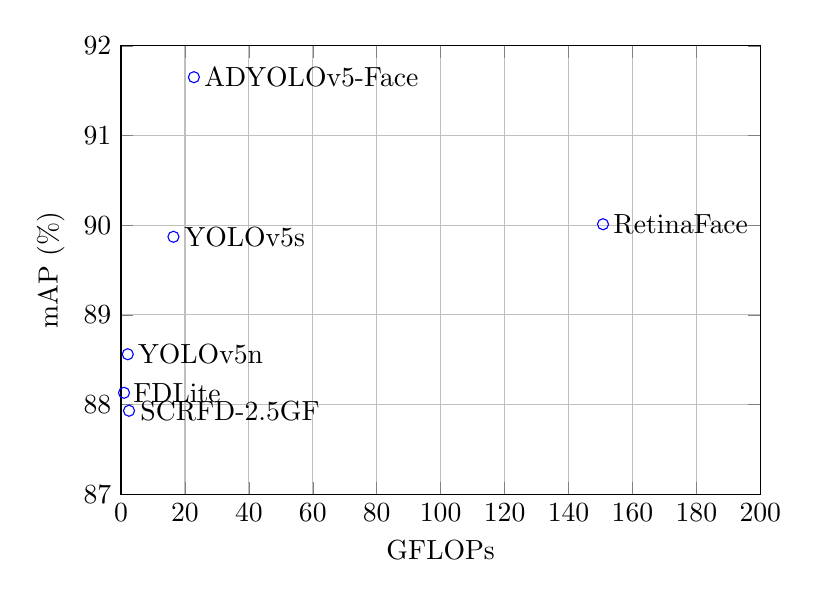
\begin{tikzpicture}
\begin{axis}[
   width=0.8\textwidth,
   height=0.6\textwidth,
   xlabel={GFLOPs},
   ylabel={mAP (\%)},
   title={},
   xmin=0, xmax=200,
   ymin=87, ymax=92,
   grid=major,
   legend pos=south east,
   scatter/classes={
       a={mark=o,draw=blue}
   }
]
\addplot[scatter,only marks,scatter src=explicit symbolic,mark size=2pt]
   coordinates {
       (22.8,91.65) [a]
       (150.79,90.01) [a]
       (16.4,89.87) [a]
       (2.5,87.93) [a]
       (0.94,88.13) [a]
       (2.111,88.56) [a]
   };
\node[anchor=west] at (axis cs:23,91.65) {ADYOLOv5-Face};
\node[anchor=west] at (axis cs:151,90.01) {RetinaFace};
\node[anchor=west] at (axis cs:16.8,89.87) {YOLOv5s};
\node[anchor=west] at (axis cs:3,87.93) {SCRFD-2.5GF};
\node[anchor=west] at (axis cs:0.8,88.13) {FDLite};
\node[anchor=west] at (axis cs:2.3,88.56) {YOLOv5n};
\end{axis}
\end{tikzpicture}
\caption{Performance vs Complexité des détecteurs de visages}
\label{fig:perf-complexity}
\end{figure}

\hspace{0.65cm}\hspace{0.65cm} L'analyse quantitative des détecteurs de visages, basée sur la visualisation comparative des performances versus ressources requises, révèle trois groupes distincts de performance-complexité : léger (<3 GFLOPs, mAP >88\%), intermédiaire (7-23 GFLOPs, mAP >89\%) et lourd (>150 GFLOPs, mAP >90\%). Le nuage de points Performance-GFLOPs démontre une distribution non-linéaire dispersée, avec ADYOLOv5-Face émergeant comme la solution la plus prometteuse, offrant les meilleures performances (mAP 91.65\%) avec une complexité modérée (22.8 GFLOPs). Cette analyse empirique identifie ADYOLOv5-Face comme solution optimale pour le marquage automatique des présences sur mobile hors ligne, avec son architecture innovante Gather-and-Distribute et ses quatre têtes spécialisées offrant une robustesse supérieure aux variations d'illumination et aux occlusions partielles. Bien que sa complexité computationnelle actuelle nécessite des optimisations, plusieurs pistes d'amélioration sont envisageables : la quantification des poids (réduction potentielle de 75\% des GFLOPs), l'élagage des connexions redondantes (gain estimé de 30-40\%), la distillation de connaissances vers une architecture plus légère (réduction possible à 5-7 GFLOPs), et l'optimisation du mécanisme GD spécifiquement pour les scénarios de salle de classe. Ces optimisations permettraient de réduire significativement l'empreinte computationnelle tout en préservant les performances supérieures qui distinguent ADYOLOv5-Face.



\begin{xltabular}{\textwidth}{>{\RaggedRight\arraybackslash}p{2cm} >{\RaggedRight\arraybackslash}p{3cm} >{\RaggedRight\arraybackslash}p{3.5cm} >{\RaggedRight\arraybackslash}p{2.5cm} >{\RaggedRight\arraybackslash}p{2.5cm} >{\RaggedRight\arraybackslash}p{2.5cm}}
\caption{Analyse comparative des méthodes de détection de visage}
\label{tab:face-detection-detailed} \\

\toprule
\textbf{Auteur}  & \textbf{Approche} & \textbf{Données d'entraînement} & \textbf{Résultats} & \textbf{Limites} \\
\midrule
\endfirsthead

\multicolumn{5}{c}{\tablename\ \thetable{} -- Suite} \\
\toprule
\textbf{Référence} & \textbf{Approche} & \textbf{Données d'entraînement} & \textbf{Résultats} & \textbf{Limites} \\
\midrule
\endhead

\midrule[\heavyrulewidth]
\multicolumn{5}{r}{\footnotesize Suite page suivante} \\
\endfoot

\bottomrule
\endlastfoot

ESSFD & 
Augmentation de données, ResNet50 pré-entraîné, taux d'apprentissage adaptatif & 
WIDER FACE & 
Précision supérieure sur trois niveaux (Easy, Medium, Hard) & 
Complexité accrue, manque détails augmentation \\
\midrule



RetinaNet & 
Points de repère du visage pour amélioration précision& 
WIDER Face, FDDB & 
95,6\% précision & 
Manque détails architecture \\
\midrule

YOLO5Face & 
Points repère 5 points, Wing loss, bloc Stem & 
WiderFace, FDDB, Webface & 
Performance pointe tous sous-ensembles & 
Manque analyse compromis \\
\midrule

FDLite & 
BLite backbone, pertes multi-tâches & 
Wider Face& 
0,24M paramètres, 0,94 GFLOPs & 
Manque données entraînement \\
\midrule


ADYOLOv5-Face & 
Gather-Distribute, tête supplémentaire, NWD, IoU & 
Wider Face, XD-Face & 
+1,1\% AP50 vs YOLOv5s & 
Manque comparaisons récentes \\




\end{xltabular}


\begin{figure}[H]
    \centering
    \begin{tikzpicture}[node distance=1.5cm and 2cm, align=center]
        % Main node
        \node[main] (B1) {\textbf{Biometric \ Systems}};
            
        % Third level nodes under B1
        \node[sub, below=of B1] (C1) {Face \\ Analysis};
        \node[sub, left=of C1] (C2) {Fingerprint \\ Recognition};
        \node[sub, right=of C1] (C3) {Iris \\ Recognition};
        
        % Fourth level nodes under C1
        \node[sub, below=of C1] (D1) {Face Detection \\ and Tracking};
        \node[sub, left=of D1] (D2) {Face \\ Recognition};
        \node[sub, right=of D1] (D3) {Facial \\ Expression \\ Analysis};
        
        % Fifth level nodes under D1
        \node[sub, below=of D1] (E1) {Machine Learning \\ Methods};
        \node[sub, left=of E1] (E2) {Classical \\ Computer Vision};
       
        
        % Sixth level nodes under D1
        \node[sub, below=of E1] (F1) {Deep Learning \\ Methods};
        \node[sub, left=of F1] (F2) {Classical \\ Machine Learning};
        
        % Seven level nodes under E1
        \node[sub, below=of F1] (G1) {Single-Stage \\ Detectors};
        \node[sub, left=of G1] (G2) {Multi-Stage \\ Architectures};
        \node[sub, right=of G1] (G3) {Attention-based \\ Models};
        
        % Additional node for multi-face detection
        \node[sub, below=of G1] (H1) {Multi-Face \\ Detection};
        
        % Solutions connected to G1
        \node[sub, below left=of H1] (S1) {YOLOv5n \\ \cite{yu2022yolofacev2scaleocclusionaware}};
        \node[sub, below=of H1] (S2) {FDLite \\ \cite{Aggarwal2024FDLiteAS}};
        \node[sub, below right=of H1] (S3) {ADYOLOv5-Face \\ \cite{electronics13214184}};
        
        % Draw arrows
        
        \draw[arrow] (B1) -- (C1);
        \draw[arrow] (B1) -- (C2);
        \draw[arrow] (B1) -- (C3);
        
        \draw[arrow] (C1) -- (D1);
        \draw[arrow] (C1) -- (D2);
        \draw[arrow] (C1) -- (D3);
        
        \draw[arrow] (D1) -- (E1);
        \draw[arrow] (D1) -- (E2);
        
        \draw[arrow] (E1) -- (F1);
        \draw[arrow] (E1) -- (F2);

        \draw[arrow] (F1) -- (G1);
        \draw[arrow] (F1) -- (G2);
        \draw[arrow] (F1) -- (G3);
        
        \draw[arrow] (G1) -- (H1);
        \draw[arrow, dashed] (H1) -- (S1);
        \draw[arrow, dashed] (H1) -- (S2);
        \draw[arrow, dashed] (H1) -- (S3);
    \end{tikzpicture}
    \caption{Techniques d'analyse pour les systèmes biométriques}
    \label{fig:biometric-analysis}
\end{figure}


\hspace{0.65cm} Cette revue de littérature démontre la pertinence de l'utilisation de YOLOv5n pour la détection multi-visages sur mobile en contexte académique. La progression depuis les fondements de l'intelligence artificielle jusqu'à cette implémentation spécifique révèle un cheminement logique, validé par des métriques quantifiables à chaque niveau de la hiérarchie technologique.


\end{onehalfspace}